\subsection{Full Cross-Benchmark Results}

\begin{table}[H]
\caption{Full cross-benchmark comparison (\%); ours reports mean $\pm$ standard deviation over five seeds.}
\label{tab:crossbench}
\centering
\scriptsize
\setlength{\tabcolsep}{4.0pt}
\resizebox{\textwidth}{!}{%
\begin{tabular}{lcccccccc}
\toprule
& \multicolumn{2}{c}{\textbf{FindingDory}} &
\multicolumn{3}{c}{\textbf{GOAT-Bench}} &
\multicolumn{3}{c}{\textbf{\pfdbench{}}}\\
\cmidrule(lr){2-3}\cmidrule(lr){4-6}\cmidrule(lr){7-9}
\textbf{Method} & \textbf{HL-SR $\uparrow$} & \textbf{HL-SPL $\uparrow$} &
\textbf{SR $\uparrow$} & \textbf{SPL $\uparrow$} &
\textbf{Repeat-SR $\uparrow$} & \textbf{First-Go SR $\uparrow$} &
\textbf{Search SR $\uparrow$} & \textbf{SPL $\uparrow$}\\
\midrule
\rowcolor{tblnav}\multicolumn{9}{c}{\emph{Open-vocabulary and lifelong navigation}}\\
VLFM \citep{yokoyama2024vlfm} & 13.42 & 10.86 & 15.79 & 5.45 & 11.82 & 20.65 & 28.36 & 24.67\\
ZSON \citep{majumdar2022zson} & 27.89 & 21.81 & 29.64 & 2.45 & 16.37 & 26.84 & 32.13 & 28.55\\
FindingDory Agent \citep{yadav2025findingdory} & 52.44 & \na & \na & \na & \na & \na & \na & \na\\
LagMemo GLUE \citep{zhou2025lagmemo} & 32.79 & 23.25 & 20.61 & 1.74 & 11.27 & 30.18 & 42.27 & 33.82\\
\midrule
\rowcolor{tblmemory}\multicolumn{9}{c}{\emph{Structured spatio-temporal memory}}\\
HOV-SG \citep{werby2024hovsg} & 21.47 & 15.20 & 28.37 & 2.23 & 12.38 & 36.46 & 52.32 & 40.61\\
DynaMem \citep{liu2024dynamem} & 30.30 & 22.78 & 14.54 & 1.71 & 15.79 & 45.33 & 81.00 & 66.83\\
\midrule
\rowcolor{tblpredict}\multicolumn{9}{c}{\emph{Predictive world and state modeling}}\\
SLaTe-PRO \citep{patel2023routine} & 18.18 & 14.53 & 9.41 & 0.99 & 6.38 & 13.00 & 36.33 & 26.37\\
SGM+NEP \citep{kurenkov2023dynamic} & 34.20 & 19.48 & 10.67 & 1.64 & 2.56 & 27.26 & 41.82 & 37.00\\
FlowMaps \citep{argenziano2026flowmaps} & 3.03 & 3.03 & 15.07 & 0.32 & 6.25 & 4.33 & 22.67 & 14.35\\
Perpetua \citep{saavedraruiz2026predictivegraphs} & 24.24 & 13.50 & 10.27 & 1.80 & 7.48 & 36.18 & 43.67 & 40.36\\
\midrule
\rowcolor{tblours} & \textbf{63.22} & \textbf{48.83} &
\textbf{35.43} & \textbf{12.98} & \textbf{19.31} & \textbf{61.32} &
\textbf{86.18} & \textbf{70.15}\\
\rowcolor{tblours}\multirow{-2}{*}{\textbf{\evolvingworldnav{} (ours)}} & $\pm 3.87$ & $\pm 2.43$ & $\pm 2.16$ &
$\pm 0.92$ & $\pm 0.68$ & $\pm 3.235$ & $\pm 2.07$ & $\pm 1.74$\\
\bottomrule
\end{tabular}
}
\end{table}
\FloatBarrier

\subsection{Cross-Environment Navigation}

\begin{table}[H]
\caption{Cross-environment navigation; SR and SPL are percentages.}
\label{tab:domains}
\centering
\scriptsize
\setlength{\tabcolsep}{3.6pt}
\resizebox{\textwidth}{!}{%
\begin{tabular}{lcccccccccc}
\toprule
& \multicolumn{4}{c}{\hdr{\textbf{Standard Simulation Worlds}}} &
\multicolumn{4}{c}{\hdr{\textbf{Photorealistic Simulation}}} &
\multicolumn{2}{c}{\hdr{\textbf{Evolving Simulation Worlds}}}\\
\cmidrule(lr){2-5}\cmidrule(lr){6-9}\cmidrule(lr){10-11}
& \multicolumn{2}{c}{\textbf{R2R-CE}} &
\multicolumn{2}{c}{\textbf{HM3D-OVON}} &
\multicolumn{2}{c}{\textbf{PointNav}} &
\multicolumn{2}{c}{\textbf{SAGE-Bench}} &
\multicolumn{2}{c}{\textbf{\pfdbench{}}}\\
\cmidrule(lr){2-3}\cmidrule(lr){4-5}\cmidrule(lr){6-7}\cmidrule(lr){8-9}\cmidrule(lr){10-11}
\textbf{Method} & \textbf{SR} & \textbf{SPL} & \textbf{SR} & \textbf{SPL} &
\textbf{SR} & \textbf{SPL} & \textbf{SR} & \textbf{SPL} & \textbf{SR} & \textbf{SPL}\\
\midrule
\rowcolor{tblmemory}\multicolumn{11}{c}{\emph{Navigation-trained or task-adapted}}\\
MTU3D \citep{zhu2025move} & 8.8 & 6.5 & 40.8 & 12.1 & 75.8 & 72.7 & 25.9 & 15.6 & 35.2 & 30.7\\
NaVid \citep{zhang2024navid} & 37.4 & 35.9 & 60.3 & 36.0 & 15.3 & 13.4 & 17.4 & 15.1 & 31.0 & 22.6\\
Uni-NaVid \citep{zhang2024uninavid} & 47.0 & 42.7 & 39.5 & 19.8 & 15.9 & 13.2 & 26.4 & 23.1 & 55.3 & 41.7\\
NaVILA \citep{cheng2024navila} & 54.0 & 49.0 & 18.3 & 9.7 & 78.4 & 77.5 & 39.0 & \textbf{34.0} & 35.2 & 30.7\\
\midrule
\rowcolor{tblnav}\multicolumn{11}{c}{\emph{Zero-shot navigation or task adapters}}\\
HSGM \citep{Li_2026_CVPR} & 47.9 & 32.8 & 40.0 & 32.5 & 37.2 & 35.3 & 11.8 & 9.4 & 17.0 & 12.5\\
VLFM \citep{yokoyama2024vlfm} & 12.0 & 9.6 & 35.2 & 19.6 & 53.0 & 42.2 & 24.4 & 18.8 & 35.0 & 25.8\\
AO-Planner \citep{chen2025affordances} & 25.5 & 16.6 & 30.9 & 22.0 & 76.6 & 74.7 & 27.4 & 19.7 & 37.0 & 29.3\\
TANGO \citep{ziliotto2025tango} & 14.3 & 9.87 & 35.5 & 19.5 & 35.8 & 33.5 & 22.7 & 14.7 & 31.0 & 23.3\\
Uni-LaViRA \citep{ding2026uni} & \textbf{60.7} & \textbf{47.7} & 60.0 & 40.5 & 81.3 & 77.7 & 35.6 & 28.7 & 65.2 & 39.4\\
MSGNav \citep{huang2026msgnav} & 11.6 & 9.4 & 48.3 & 27.0 & 37.2 & 34.8 & 23.5 & 17.5 & 26.7 & 19.6\\
\rowcolor{tblours}\textbf{\evolvingworldnav{} (ours)} & 55.8 & 43.1 &
\textbf{64.2} & \textbf{51.7} & \textbf{86.2} & \textbf{79.8} &
\textbf{42.4} & 32.1 & \textbf{86.6} & \textbf{68.2}\\
\bottomrule
\end{tabular}
}
\end{table}
\FloatBarrier

\subsection{Real-World Search Case}

\begin{figure}[H]
    \centering
    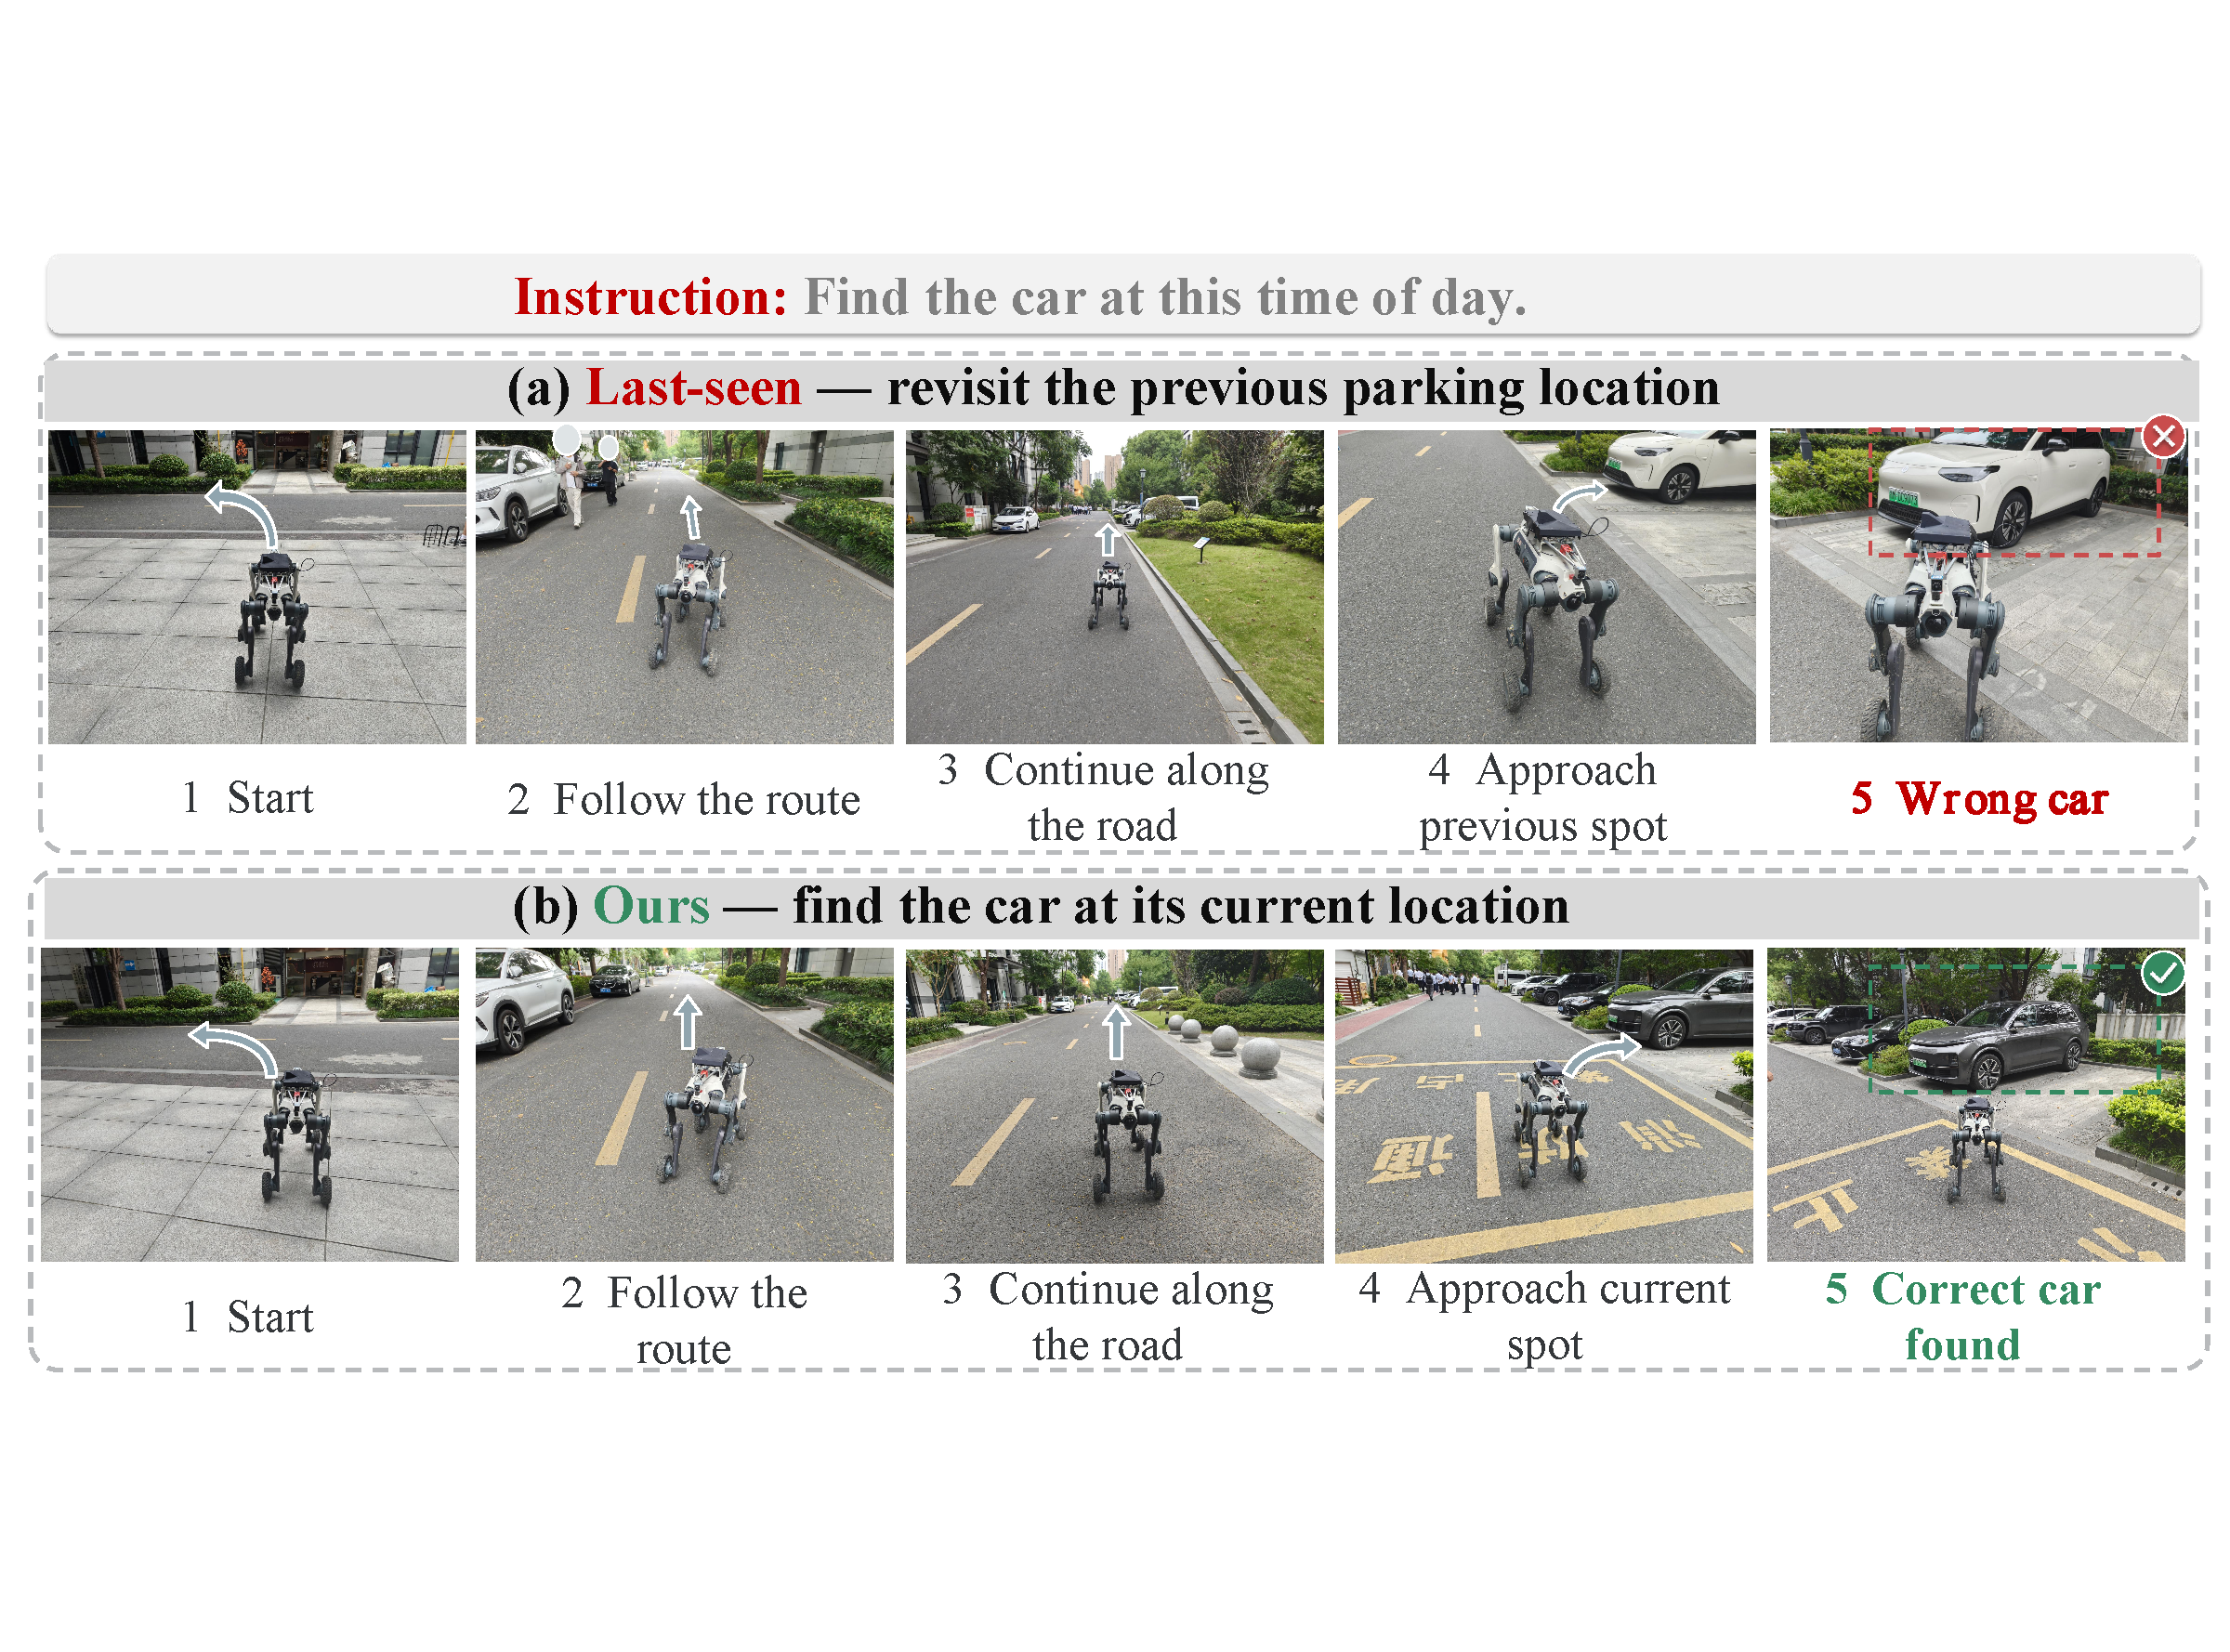
\includegraphics[width=\textwidth]{figures/Real_World_Case_third_1.pdf}
    \caption{Outdoor search under stale and predictive memories.}
    \label{fig:real-world-car-case}
\end{figure}

\subsection{Full Prediction Results and Calibration}
\label{app:full-prediction-results}

\begin{table}[H]
\centering
\scriptsize
\setlength{\tabcolsep}{3pt}
\caption{Full prediction-only results on temporal changed-only ($n=322$) and LOSO
change-balanced queries ($n=644$). Ours reports mean $\pm$ standard deviation
over five seeds; Top-1 is in percent, while MRR and NLL are unscaled.}
\label{tab:predictors-full}

\resizebox{\linewidth}{!}{%
\begin{tabular}{lrrrrrr}
\toprule
Predictor
& Temporal Top-1 $\uparrow$
& MRR $\uparrow$
& NLL $\downarrow$
& LOSO Top-1 $\uparrow$
& MRR $\uparrow$
& NLL $\downarrow$ \\
\midrule

Uniform Random
& 9.32
& 0.2607
& 2.4509
& 11.96
& 0.3050
& 2.2980 \\

Last Seen
& 0.00
& 0.1699
& 3.4011
& 50.00
& 0.5850
& 1.8825 \\

Object Frequency
& 30.75
& 0.5476
& 1.7397
& 50.47
& 0.6441
& 1.8455 \\

Time Frequency
& 33.85
& 0.5462
& 1.8400
& 49.53
& 0.6166
& 1.6455 \\

Markov
& 18.94
& 0.4435
& 2.3772
& 49.38
& 0.6286
& 1.6982 \\

Activity-Markov
& 25.16
& 0.4582
& 2.2436
& 49.84
& 0.6221
& 1.6183 \\

Random Forest
& 20.50
& 0.4851
& 1.9181
& 58.07
& 0.7283
& 1.1441 \\

Packed MLP
& 29.50
& 0.5225
& 2.1036
& 58.07
& 0.7173
& 1.3105 \\

GRU
& 32.61
& 0.5471
& 1.8279
& 54.04
& 0.7016
& 1.2558 \\

Original gated Transformer
& 34.16
& 0.5586
& 1.7292
& 51.71
& 0.6884
& 1.3157 \\

Shared semantic prior
& 36.02
& \textbf{0.5957}
& 1.5766
& 59.47
& 0.7462
& 1.0448 \\

\rowcolor{tblours}
& \textbf{38.24}
& \textbf{0.5971}
& \textbf{1.4925}
& \textbf{61.18}
& \textbf{0.7523}
& \textbf{0.9778} \\
\rowcolor{tblours}\multirow{-2}{*}{\textbf{Ours}}
& $\pm 1.42$
& $\pm 0.0291$
& $\pm 0.0867$
& $\pm 4.53$
& $\pm 0.0176$
& $\pm 0.0228$ \\

\bottomrule
\end{tabular}%
}
\end{table}

\begin{figure}[H]
    \centering
    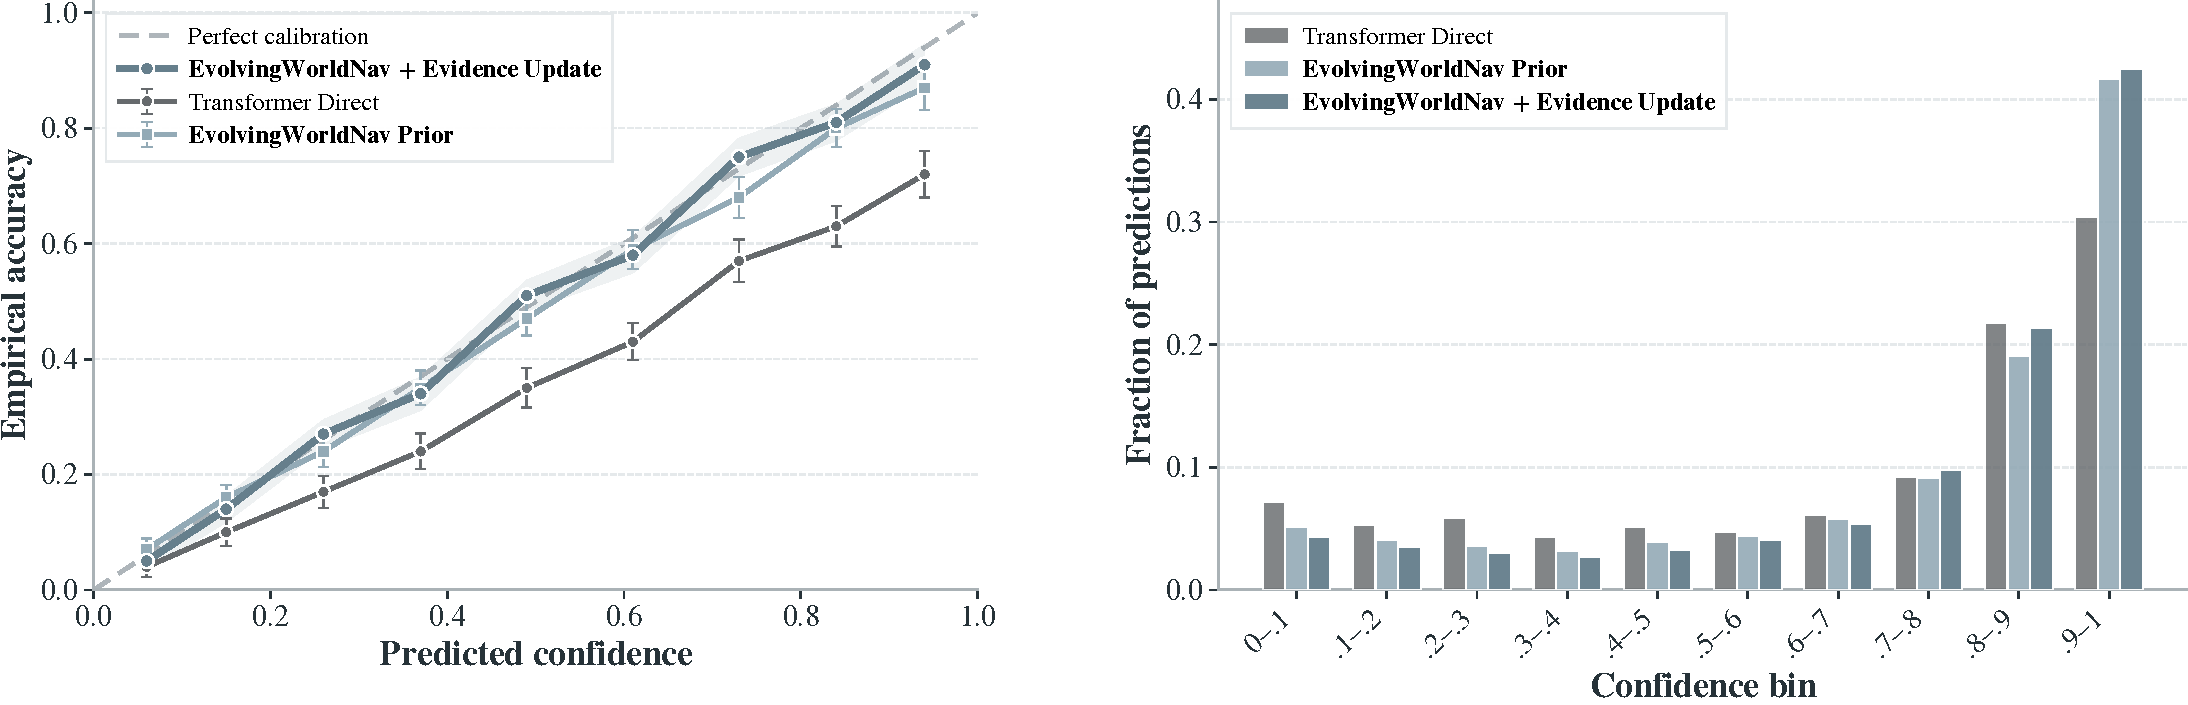
\includegraphics[width=\textwidth]{figures/calibration_current_state_belief_2panel.pdf}
    \caption{Calibration of current-state beliefs before and after evidence updates.}
    \label{fig:belief-calibration}
\end{figure}
\FloatBarrier
